%class
	\documentclass{beamer}

%template
	\usetheme{HannoverSalman}
	\setbeamertemplate{navigation symbols}{}
	%\setbeamertemplate{footline}{\centering{\insertframenumber/\insertpresentationendpage}}
	%\setbeamertemplate{footline}{\hspace*{.5cm}\scriptsize{\hfill\insertframenumber\hspace*{.5cm}}} 


%packages
	\usepackage{amsmath, amssymb, graphicx,cancel}
	\usepackage[absolute,overlay]{textpos}
	\usepackage{subfigure}
	\usepackage{caption}\captionsetup{labelformat=empty,labelsep=none}
	\usepackage{geometry}
	\geometry{verbose}
	\usepackage{color}
	\usepackage{xmpmulti}
	\usepackage[3D]{movie15}
	\usepackage{hyperref}
%	\usepackage{bookmark}
	\usepackage[open,openlevel=4,atend]{bookmark}
	%\bookmarksetup{color=blue}
	\usepackage{multirow}
	\usepackage[style=numeric,defernumbers, authoryear]{biblatex}
	%\usepackage[square,sort]{natbib}
	%\usepackage{fancyhdr}%\pagestyle{fancy} 

	
	\hypersetup{bookmarksdepth = 4}


%citations files
	\bibliography{MyCitations}

%logoCSIPCPL
    \setlength{\TPHorizModule}{1mm}
    \setlength{\TPVertModule}{1mm}
    \newcommand{\logoCSIPCPL}
    {
    	\begin{textblock}{1}(100,2) %(100,85)  for bottom
    		\includegraphics[width=1.5cm]{figs/logo_CSIP}
    	\end{textblock}
    	
	\begin{textblock}{1}(117,1) %(117,85)  for bottom
    		\includegraphics[width=1.0cm]{figs/logo_CPL}
    	\end{textblock} 
    }

%logo evolution
    \newcommand{\logoEvolution}
    {    	
	\begin{textblock}{1}(110,1) %(117,85)  for bottom
    		\includegraphics[width=0.65in]{figs/logo_evolution.pdf}
    	\end{textblock} 
    }

%logo Qualcomm
    \newcommand{\logoQualcomm}
    {
    	\begin{textblock}{1}(110,2) %(100,85)  for bottom
    		\includegraphics[width=1.5cm]{figs/logo_qualcomm.jpg}
    	\end{textblock}
    }
%logo Qualcomm (long)
    \newcommand{\logoQualcommllong}
    {
    	\begin{textblock}{1}(0,0) 
    		\includegraphics[width=1.25in]{figs/logo_qualcomm_long.jpg}
    	\end{textblock}
    }

%logo Tech Tower
    \newcommand{\logoTechTower}
    {
    	\begin{textblock}{1}(0,0) 
    		\includegraphics[width=1.25in]{figs/logo_TechTower.jpg}
    	\end{textblock}
    }

%logo tree
    \newcommand{\logoTree}
    {
    	\begin{textblock}{1}(0,0) 
    		\includegraphics[width=1.25in]{figs/logo_tree.jpg}
    	\end{textblock}
    }
%page numbers
    \newcommand{\mypagenum}
    {
    	\begin{textblock}{1}(1,94) 
		{\tiny \color[rgb]{0.2,0.2,1}\insertframenumber} %\insertframenumber,\insertpresentationendpage, \inserttotalframenumber
    	\end{textblock}
    }
%my footnote citation
	\newcommand{\myFootnoteCitation}[2]
	{
		\footnote{\tiny \citeauthor{#1}, \emph{#2}, \citeyear{#1}.}  %\citeauthor{#1}, \citetitle{#1}, #2 \citeyear{#1}.
	}
%my refer to citation
	\newcommand{\mycite}[1]
	{
		\emph{\citeauthor{#1} (\citeyear{#1})}
	}
%my footnote website citation
	\newcommand{\myFootnoteWebsiteCitation}[1]
	{
		\footnote{\tiny \citeauthor{#1}}
	}

\let\thefootnote\relax\footnotetext{Footnotetext without footnote mark}


%section underline
%\newcommand{\tmpsection}[1]{}
%\let\tmpsection=\section
%\renewcommand{\section}[1]{\tmpsection{\underline{#1}}}



%commands
	\newcommand{\likelihood}{p(Z_k| x_k) }						%likelihood
	\newcommand{\prior}{p(x_k)  } 								%prior
	\newcommand{\posterior} {p(x_k| Z_k)}						%posterior
	\newcommand{\prediction} {p(x_k| Z_{k-1})}					%prediction
	\newcommand{\update} {p(x_k|Z_k)}							%update
	\newcommand{\observations} {p(Z_k)}						%observations
	\newcommand{\prevobservations} {p(Z_{k-1})}				%previous observations
	\newcommand{\dxpk} {dx_{k-1}}							%dx_{k-1}
	\newcommand{\ChapKolm}{\int{p(x_k| x_{k-1})p(x_{k-1}|Z_{k-1})} \dxpk} %Chapman Kolmogorov

	%algorithm specific: JPDAF
	\newcommand{\likelihoodJPDAF}{p(Z_k| \chi, m, Z_{k-1}) }		%1. likelihood
	\newcommand{\priorJPDAF}{p(\chi|m, Z^{k-1}} 				%2. prior	
	\newcommand{\observationsJPDAF} {p(Z_k}					%3. observations
	\newcommand{\posteriorJPDAF} {p(\chi| Z_k)}					%4. posterior

%environments
	\newenvironment{changemargin}[2]
	{
	  	\begin{list}{}
		{
			\setlength{\topsep}{0pt}%
			\setlength{\leftmargin}{#1}%
			\setlength{\rightmargin}{#2}%
			\setlength{\listparindent}{\parindent}%
			\setlength{\itemindent}{\parindent}%
			\setlength{\parsep}{\parskip}%
		}
	  	\item[]
		}
		{\end{list}
	}
%figures

%colors
\definecolor{darkgreen}{rgb}{0,0.5,0}

%personal details
	\author{Salman Aslam}
	\institute{Advisor, Dr Christopher Barnes (ECE)\\Co-advisor, Dr Aaron Bobick (CoC)\\Georgia Institute of Technology}
	\date{}

\begin{document}
\newboolean{Slides_or_Talk}
\setboolean{Slides_or_Talk}{true}

%####################################################################################################
\title{Better Computer Vision \\ Under Video Compression,\\ An Example Using Mean Shift Tracking}
%####################################################################################################
\begin{frame}[plain]\logoTechTower
	\titlepage
\end{frame}

\begin{frame}\frametitle{Outline}\logoTechTower\logoCSIPCPL\mypagenum
	\tableofcontents
\end{frame}

%####################################################################################################
\section{Introduction}
%####################################################################################################

\begin{frame}
\frametitle{Introduction}
\framesubtitle{goal}
\logoCSIPCPL\mypagenum
\ifthenelse{\boolean{Slides_or_Talk}}
{
	We want to run some computer vision algorithm (e.g. tracking) on compressed video.
	\begin{itemize}
		\item We would like the results of the algorithm (e.g. track positions) to be as close as possible to results generated if the algorithm were run on uncompressed video.
	\end{itemize}
	\begin{figure}		
		\includegraphics[width=0.9\textwidth]{figs/ICIP2009_ProblemStatement.pdf}
	\end{figure}
}
{
Initial scenario:  There is a camera in the field.  It does some processing on the raw video it captures.  It transmits both the raw video and the processed information to a central server.  This is the standard configuration.
\newline
\newline
New configuration: There is a requirement now that the processing done by the camera needs to be done at the server.  Furthermore, the camera is only allowed to transmit compressed video to the server, and not its results.  In this new configuration, the server needs to do its processing on compressed video.  This is where we step in and find ways of transforming the raw video in such a manner that when it is compressed and sent to the server, processing results at the server are reasonably close to processing results from raw video.
}
\end{frame}





%===================================
\subsection{Possible solutions}
%===================================
\begin{frame}
\frametitle{Introduction}
\framesubtitle{possible solutions}
\logoCSIPCPL\mypagenum
\ifthenelse{\boolean{Slides_or_Talk}}
{
	\begin{enumerate}
		\item Codec based solution
			\begin{itemize}
				\item custom codec
				\item standard codec
					\begin{itemize}
						\item metadata support, e.g. MPEG-4
						\item intelligently vary quantization parameter $Q_p$, or quantization matrices
					\end{itemize}
			\end{itemize}
		\item Signal processing based solution
			\begin{itemize}
				\item Vary input signal intelligently to make it robust to degradations in the encoding/decoding process
			\end{itemize}
	\end{enumerate}
}
{
In order to achieve this goal, we look at what possible solutions we can come up with.  The most straightforward solution is to build a custom codec that preserves the information we need.  However, this is not very practical as we will have to build a custom codec for every application.  We could also use a codec with metadata support, like MPEG-4.  In this manner, processing results by the field camera can be embedded within the compressed video stream.  The disadvantage of this approach is that this feature is not available in the commonly used MPEG-4 profiles.  We could also vary the quantization parameter $Q_p$ intelligently, and this is the topic of our next paper.  The final approach could be to change our input signal slightly so that it remains 'reasonably' close to the original video for a human observer, but is more robust to degradations in the MPEG-4 process.
}
\end{frame}



%===================================
\subsection{Our approach}
%===================================
\begin{frame}
\frametitle{Introduction}
\framesubtitle{our approach} 
\logoCSIPCPL\mypagenum
\ifthenelse{\boolean{Slides_or_Talk}}
{
	{\color{red}Signal processing based solution} \\ 
	Calculus of Variations problem, with functional J
%	\begin{equation*}
%		 \min_{g} J(g)=\iint_D \left\|f(I) - f(\hat{g}(I)) \right\|_2  +  \lambda \left\|p(I) -  p(\hat{g}(I)) \right\|_2 dxdy
%	\end{equation*}
	\begin{figure}
		\includegraphics[width=1.0\textwidth]{figs/ICIP2009_MathematicalFormulation.pdf}
	\end{figure}
	$D$ is the domain of the image\\
	$s(.)$ is an image similarity measure
}
{
Our next step is to try to formulate our problem in mathematical terms.  We can look at this problem as a calculus of variations problem.  We are trying to find a mapping, out of all possible mappings, that when applied to the input signal, will help it preserve certain characteristics of interest, even when it undergoes compression and decompression.  For instance, in a color tracking application, we want the color distributions of our targets of interest to undergo minimal distortion.  In this paper, we work with Mean Shift Tracking on the Hue channel (HSV space).  Our goal is to preserve the hue distribution of our targets of interest.
\newline
\newline
Mean Shift Equations given on this slide show how to compute the target center.  These equations are applied iteratively until they converge.  Convergence takes about 3 or 4 iterations.  It is clear that the computational complexity of these equations is low.  Moreover, the number of iterations, i.e. 3 or 4, is small.
}
\end{frame}






\begin{frame}
\frametitle{Introduction}
\framesubtitle{Our approach (cont.)}
\logoCSIPCPL\mypagenum
	\begin{itemize}
		\item {\color{red}Computer vision algorithm, $f(.)$:} \\ Mean shift tracking on hue space
		\item {\color{red}Preserving information,  $g(.)$:} \\ Smooth out variations in hue space
			\begin{itemize}
				\item A segmentation method can be used to manipulate the hue distribution
				\item Modified stochastic gradient descent algorithm to find locally optimal parameters
				\item Pick a local parameter space at random and optimize parameters locally
			\end{itemize}
	\end{itemize}
	\vspace{0.1in}
	\begin{figure}
		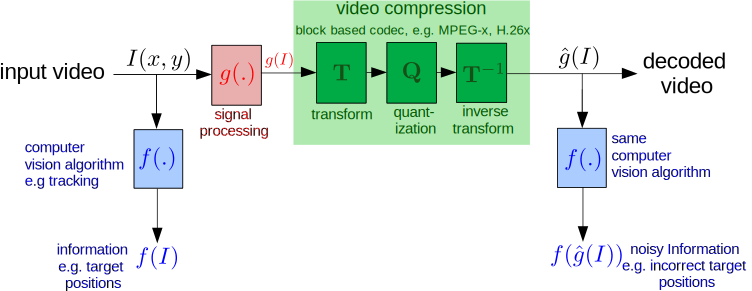
\includegraphics[width=0.8\textwidth]{figs/ICIP2009_SolutionThroughSigProc.pdf}
	\end{figure}
\end{frame}

%===================================
\subsection{Theoretical background}
%===================================
\begin{frame}
\frametitle{Mean shift filtering}
\framesubtitle{notation}
\logoCSIPCPL\mypagenum
	\begin{itemize}
		\item {\color{red}$N$}: number of data points
		\item {\color{red}$D$}: number of dimensions
	 	\item {\color{red}$p(x)$}: distribution of {\color{red}$x$}
		\item {\color{red}$R$}: small region containing {\color{red}$K$} data points (a subset of all the data points in $x$)
		\item {\color{red}$V$}: volume of $R$
		\item {\color{red}$P$}: each point in $x$ has probability $P$ of falling in $R$, where
			\begin{equation*}
				P=\int_R p(x)dx
			\end{equation*}
		\item {\color{red}\text{bin}$(K|N,P)$}: binomial distribution for $K$
		\item {\color{red} $k(u)$}: unit square centered on origin, a Parzen window
			\begin{equation*}
				k(u) = 
				\left\{ 
				\begin{array}{rl}
					1\text{,} &  |u_i|<1/2 \ \ \ \ \ \ \ \ \ i=1,\ldots, D\\ 
					0\text{,} &  \mbox{otherwise}
				\end{array}
				\right.
			\end{equation*}
	\end{itemize}
\end{frame}




\begin{frame}
\frametitle{Mean shift filtering}
\framesubtitle{adaptive gradient ascent}
\logoCSIPCPL\mypagenum
	\begin{figure}				
		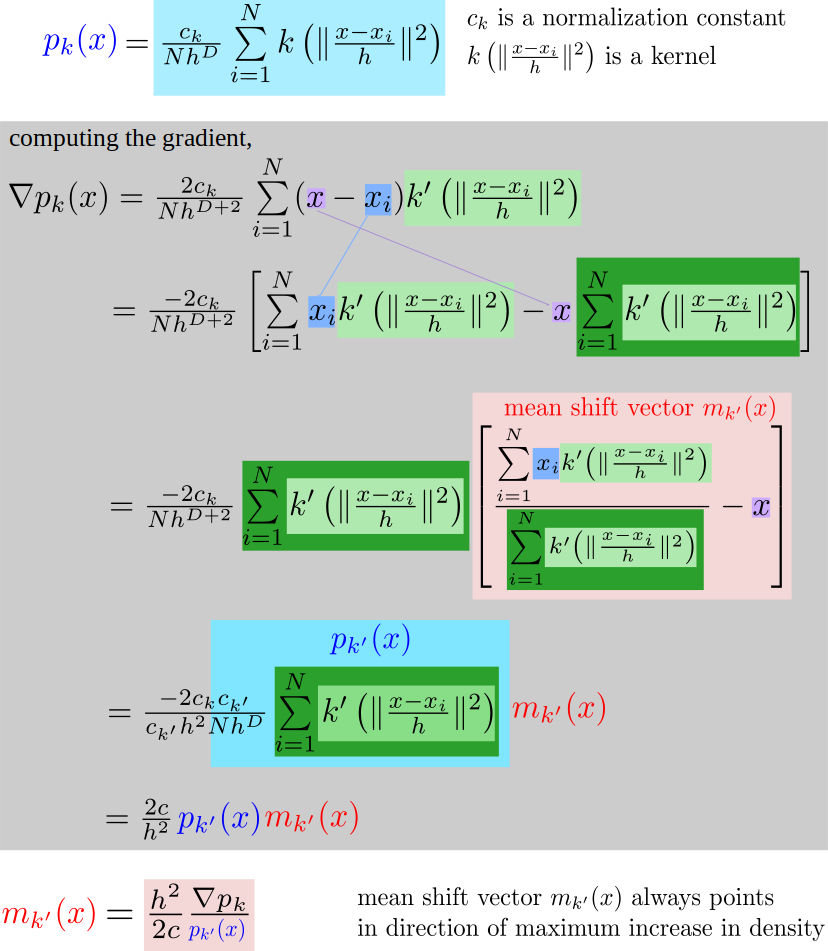
\includegraphics[height=.85\textheight]{figs/PRML_meanShift.pdf}
	\end{figure}
\end{frame}





\begin{frame}
\frametitle{Mean shift filtering}
\framesubtitle{simplification with uniform kernel}
\logoCSIPCPL\mypagenum
	New target center, $x_c$ and $y_c$ are computed as,
	\begin{align*}
		\label{eq:MeanShiftEquations}
		M_{00}&=\sum_x\sum_yI(x,y)		\\
		M_{10}&=\sum_x\sum_yxI(x,y)		\\
		M_{01}&=\sum_x\sum_yyI(x,y)		\\
		x_c&=\frac{M_{10}}{M_{00}}		\\
		y_c&=\frac{M_{01}}{M_{00}}
	\end{align*}
\end{frame}



\begin{frame}
\frametitle{Mean shift segmentation}
\framesubtitle{steps}
\logoCSIPCPL\mypagenum
	\begin{enumerate}				
		\item {\color{red}Mean shift filtering}
			\begin{itemize}
				\item For a pixel, compute its mean shift vector
				\item This mean shift vector ends at a mode of the density
				\item Repeat for all pixels, now you have a bunch of modes
				\item The set of all locations that converge to the same mode defines the  \emph {basin of attraction} of that mode
			\end{itemize}
		\item  {\color{red}Merge basins of attraction}
			\begin{itemize}
				\item Merge (i.e. prune) modes that are close to each other, and corresponding basins of attraction
			\end{itemize}
	\end{enumerate}
\end{frame}




\begin{frame}
\frametitle{Mean shift segmentation}
\framesubtitle{example\footnote{Comaniciu et. al., 2002}}
\logoCSIPCPL\mypagenum
	\begin{itemize}				
		\item 7 pruned nodes
		\item 7 corresponding basins of attraction (i.e. clusters, or segmented regions)
	\end{itemize}
	\begin{figure}
		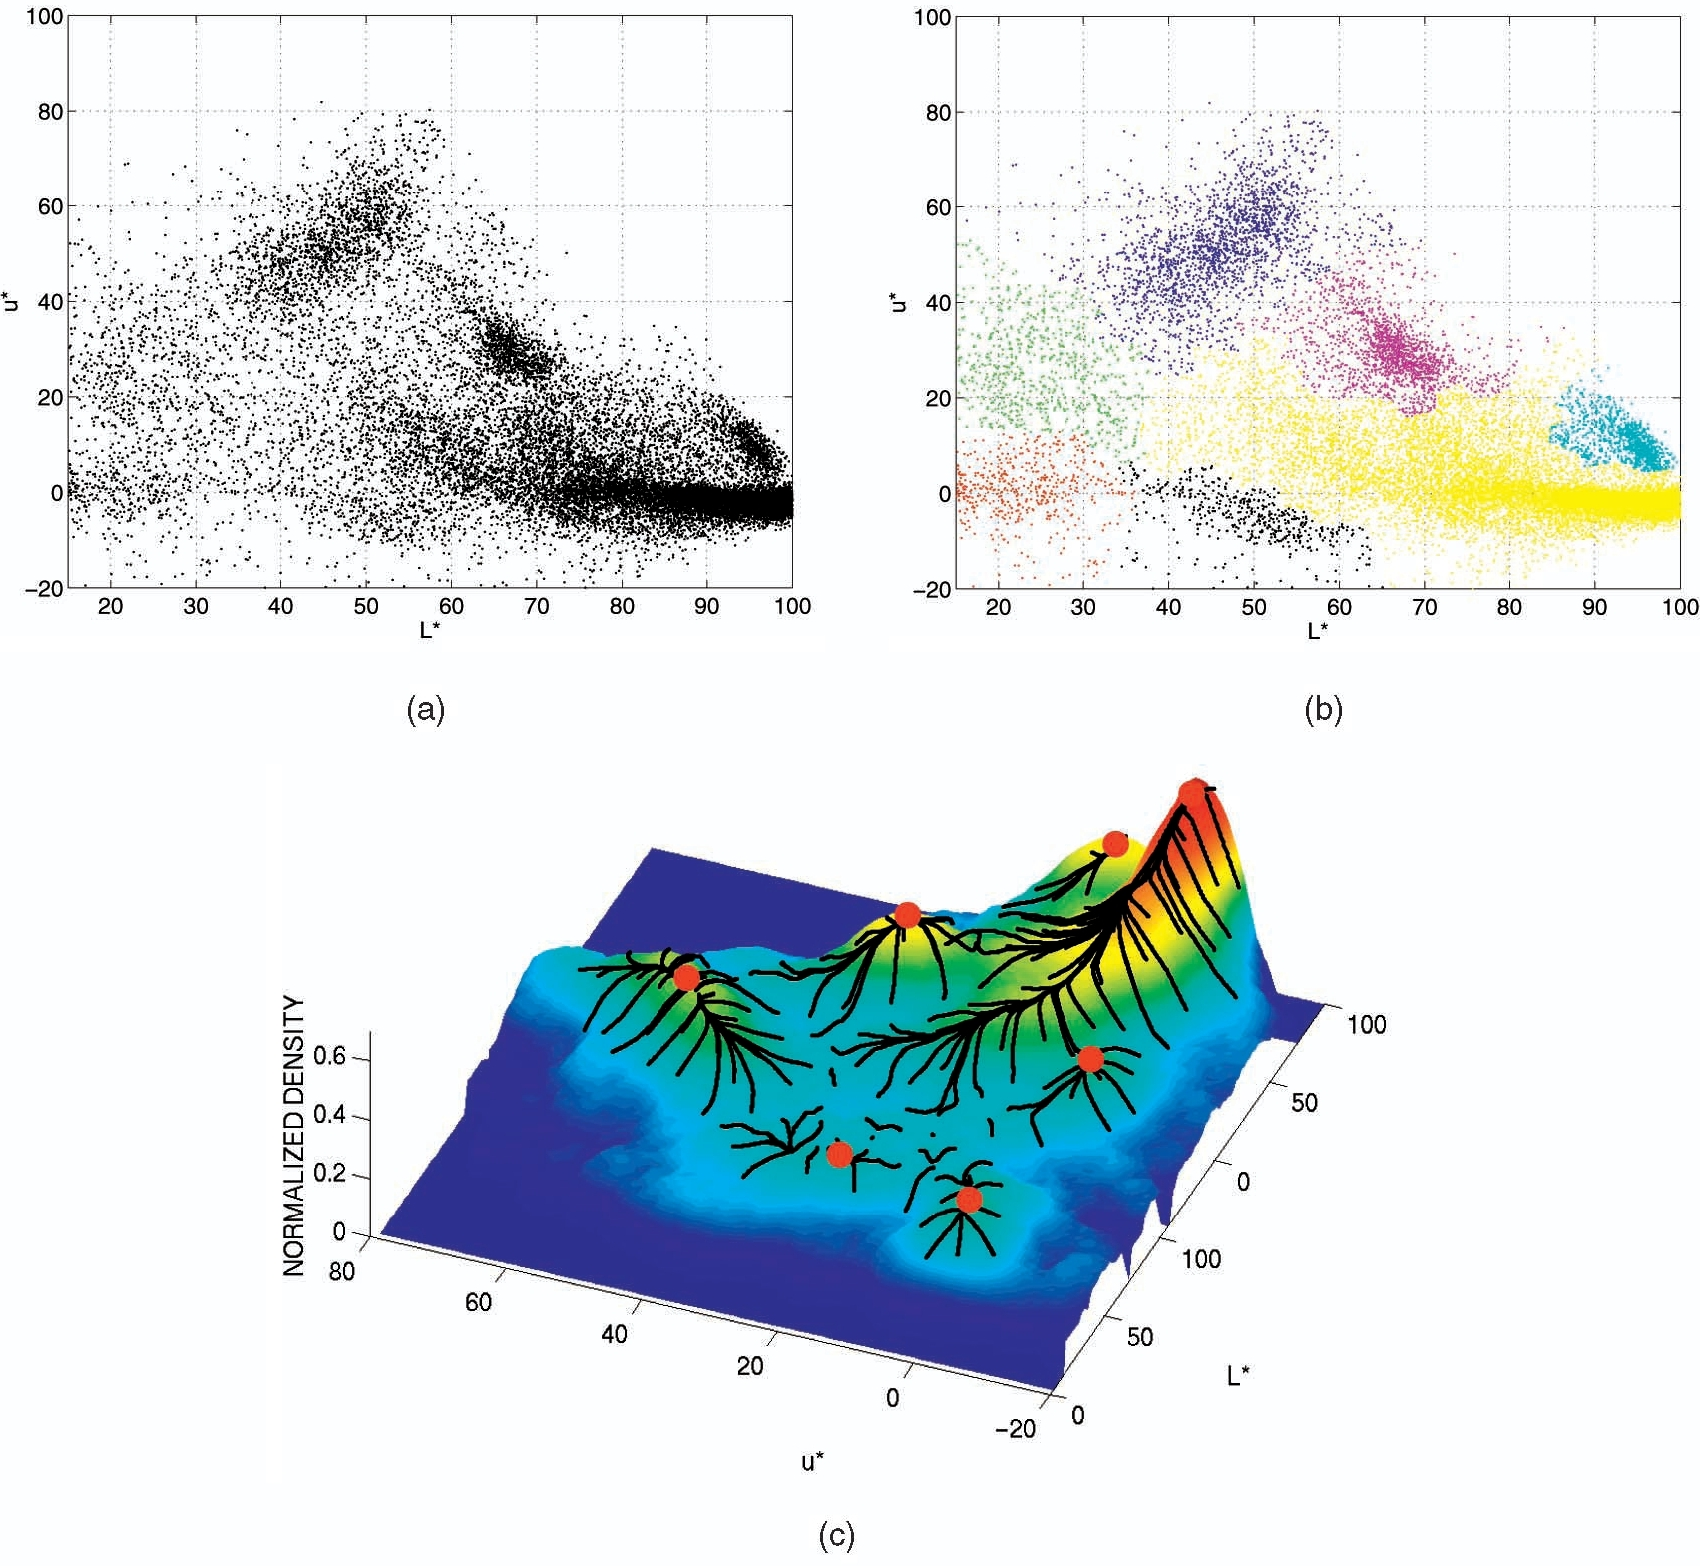
\includegraphics[height=0.6\textheight]{figs/PRML_meanShift2.pdf}
	\end{figure}
\end{frame}




%####################################################################################################
\section{Experiments}
%####################################################################################################

\begin{frame}
\frametitle{Experimental Setup} 
\logoCSIPCPL\mypagenum
\ifthenelse{\boolean{Slides_or_Talk}}
{
	\begin{figure}
		\includegraphics[width=1.0\textwidth]{figs/ICIP2009_ExperimentalSetup.pdf}
	\end{figure}
}
{
In this slide, we give our experimental setup.  The ground truth is computed by running the Mean Shift tracking algorithm on raw video.  This gives us the standard results that we would like to get even when tracking is run on compressed video.  Tracker 1 (baseline) produces results if tracking is done on the compressed video.  We would like to improve these results and bring them closer to the ground truth results.  Finally, in tracker 2, we apply Mean Shift segmentation to the input, and then run tracking on the compressed video.
}
\end{frame}



%####################################################################################################
\section{Results}
%####################################################################################################
\begin{frame}
\frametitle{Results} 
\framesubtitle{PETS2001} 
\logoCSIPCPL\mypagenum
\ifthenelse{\boolean{Slides_or_Talk}}
{
	\begin{itemize}
		\item person tracking
		\item sparse background
		\item target occluded by object (car) with similar color distribution
	\end{itemize}
	\begin{figure}
		\includegraphics[width=1.0\textwidth]{figs/ICIP2009_PETS2001_FN_00592_snapshotVVG.pdf}
	\end{figure}
}
{
In PETS2001, we track a person in a sparse background as she gets occluded by a car with a similar color distribution.  In PETS2007 (next slide), we track a bag in a dense environment.  These two scenarios were chosen since they are quite different and would provide a better test of our approach.  Additionally, in both cases, the tracked object is occluded by another object with a similar color distribution.  This of course, presents one of the most significant challenges in tracking applications. 
\newline
\newline
The top left figure shows ground truth, the top right shows tracker 1, i.e. baseline, and bottom right shows tracker 2.  Notice that tracker 2 keeps track while tracker 1 looses track.
}
\end{frame}







\begin{frame}
\frametitle{Results}
\framesubtitle{PETS2007}
\logoCSIPCPL\mypagenum 
\ifthenelse{\boolean{Slides_or_Talk}}
{
	\begin{itemize}
		\item object (bag) tracking
		\item dense background
		\item target occluded by object with similar color distribution
	\end{itemize}
	\begin{figure}
		\includegraphics[width=1.0\textwidth]{figs/ICIP2009_PETS2007_FN_00340_snapshotVVG.pdf}
	\end{figure}
}
{
Again, the top left figure shows ground truth, the top right shows tracker 1, i.e. baseline, and bottom right shows tracker 2.  And again, tracker 2 keeps track while tracker 1 looses track.
}
\end{frame}









\begin{frame}
\frametitle{Results}
\framesubtitle{tracking error}
\logoCSIPCPL\mypagenum 
\ifthenelse{\boolean{Slides_or_Talk}}
{
	\begin{columns}
		\begin{column}{1.8in}
			\begin{center}
				PETS2001
			\end{center}
			\begin{figure}
				\includegraphics[width=1.0\textwidth]{figs/ICIP2009_SLIDES_Accuracy_PETS2001.pdf}
			\end{figure}
		\end{column}
		\begin{column}{1.8in}
			\begin{center}
				PETS2007
			\end{center}
			\begin{figure}
				\includegraphics[width=1.0\textwidth]{figs/ICIP2009_SLIDES_Accuracy_PETS2007.pdf}	
			\end{figure}
		\end{column}			
	\end{columns}
	\begin{itemize}
		\item Original tracker can lose track while improved tracker remains within an average of 5 pixels of target center
		\item Same bitrate
		\item PSNR drop for entire image is around 2 dB
		\item PSNR drop inside ROI is between 2 and 11 dB
	\end{itemize}
}
{
Here, we show that at different values of $Q_p$, tracker 2 does indeed perform better than the baseline tracker, i.e. Tracker 1.  
}
\end{frame}











%####################################################################################################
\section{Conclusions}
%####################################################################################################

\begin{frame}\frametitle{Conclusions} \logoCSIPCPL\mypagenum
	\begin{enumerate}
		\item It is possible to preserve information in a compressed video signal for a given application
			\begin{itemize}
				\item In this work, we focused on tracking at low bit-rates
				\item challenging scenes were used
				\item person or a bag was tracked after being occluded by another object with similar color distribution
			\end{itemize}
		\item Tracking accuracy was improved in 95 \% of the cases tested
			\begin{itemize}
				\item average PSNR drop of 5dB inside the segmentation window for a given bitrate
			\end{itemize}
	\end{enumerate}
\end{frame}


%####################################################################################################
%####################################################################################################
%\bibliographystyle{ieee}
%\bibliography{c:/salman/work/writing/MyCitations}
\end{document}
%####################################################################################################

%####################################################################################################



%----------------------------------------------------------------------------------
%\section{Introduction} 
%----------------------------------------------------------------------------------
%%#################
%\frame{\frametitle{blocs}
%%#################
%
%\begin{block}{title of the bloc}
%bloc text
%\end{block}
%
%\begin{exampleblock}{title of the bloc}
%bloc text
%\end{exampleblock}
%
%
%\begin{alertblock}{title of the bloc}
%bloc text
%\end{alertblock}
%}